% Chapter 1

\chapter{Introduction} % Main chapter title

\label{Chapter1} % For referencing the chapter elsewhere, use \ref{Chapter1} 

%----------------------------------------------------------------------------------------

% Define some commands to keep the formatting separated from the content 
% \newcommand{\keyword}[1]{\textbf{#1}}
% \newcommand{\tabhead}[1]{\textbf{#1}}
% \newcommand{\code}[1]{\texttt{#1}}
% \newcommand{\file}[1]{\texttt{\bfseries#1}}
% \newcommand{\option}[1]{\texttt{\itshape#1}}

%----------------------------------------------------------------------------------------

% =========================================================== %
%                 Section: Spatial navigation                 %
% =========================================================== %

\section{Spatial navigation}
\label{chap1:sec1:spatial_navigation}

The interaction between organisms and the environment is the core of life and evolution. This interaction happens at different levels with different objectives and outcomes. 
From the behavioural point of view, organisms have evolved to be able to perceive different aspects of the environment, interpret them and act in consequence. 
The more we move forward in evolution the more sophisticated and complex resources and behaviours we observe, being the nervous system, perhaps, the mayor and most interesting exponent of this. 

One of the most fundamental aspects of such interaction consists on being able to move and navigate through the environment.
A functional navigation system has to achieve a series of very difficult tasks that include the integration of information from different sensory modalities and coordination with the motor system, together with higher order cognitive processes like proprioception and goal directed activity in a flexible and dynamic way.

Spatial navigation has been extensively studied in the last 50 years, in particular, in the mammalian brain. 
The seminal work of John O'Keefe during the 1970s on rats lead to the hypothesis of a \textit{cognitive map} [REF to the book] as the way the brain solves the challenge of spatial navigation and, importantly, to experimental corroborations of the possible neuronal implementation of it. 
Unexpectedly such implementation involved the activity of specialized cells in a restricted area of the brain: \hyperref[chap1:sec:1:subsec1:hippocampus]{\textbf{The Hippocampus}}.

According to the \textit{cognitive map} theory, cells in the Hippocampus would receive inputs conveying information about sensory cues related to environmental stimuli, calculate the animal's position in space and consequently predict subsequent positions and trajectories depending on goal, inferred distances and directions. 
The ability of the internal navigation system to calculate trajectories and predict future positions represents the essence of learning in the cognitive map and has several implications regarding the internal structure, what kind of computations and types of cells should be find in the Hippocampus.

In the next sections we will summarize the anatomy and function of the Hippocampus and the different types of information encoding cells found to be present in the hippocampal navigation system.

% =========================================================== %
%                    Subsection: Hippocampus                  %
% =========================================================== %
\subsection{The Hippocampus}
\label{chap1:sec:1:subsec1:hippocampus}
Although hippocampal anatomy and connectivity has been extensively studied for decades, it's understanding and it's relationship with function is far from being completely elucidated [reference to something about discrepancies or open questions]. 
Here we will briefly described the canonical hippocampal circuit, it's constituents, structure and connectivity, paying special attention to the flow of information in the circuit.

The mammal Hippocampus is a seahorse-shaped (hence the name) brain structure located underneath the temporal lobe of the neocortex.
All mammals have a structure that could be identify as an Hippocampus, moreover, it is possible to identify a homologue of the mammalian hippocampus in all vertebrates [reference to the okeefe book, Ariens Kappers, Huber, and Crosby 1936, pp. 1248-1255, Heier 1948, Crosby, Dejong, and Schneider 1966].
It's interesting to note though, that besides the difference in structure, the Hippocampus homologues can play an entire different functional role.
The grid like structure of the Hippocampus could be thought as a general mapping structure that accomplish different functions depeneding on the species. 
In the mouse and rat, which is the case that concerns this work, is thought to be used as a spatial mapping structure, as discussed before.

In this animal the Hippocampus occupies a large portion of the forebrain and represents the paradigm of the simple cortex, consisting primarily of one basic cell type, the pyramidal or granule cells, and its asociated interneurons, the basket cells [Figure \ref{fig:chap1:spatialnavigation}b]. 
In fact, a horizontal section through the posterior arch of the hippocampus shows the transition form the six layered complex structure of the entorhinal neocortex to the three layered hippocampal formation through the \textit{subiculum} [Figure \ref{fig:chap1:spatialnavigation}a].

The hippocampal structure can be divided in two U-shaped interlocking sectors, the \textit{hippocampus proper} and the \textit{dentate gyrus}. 
The hippocampus proper can, in turn, be divided in 4 subfields CA1-4 [Lorente de No 1934]. 
CA stands for \textit{cornu ammonis}, another shape-like reference. 
Following the structured layer of principal neurons, CA1 appears first as the main output region of the hippocampus, followed by CA2-3 in the regio inferior and finally CA4 represents the scattered cells inside the hilus of the dentate gyrus [see Figure \ref{fig:chap1:spatialnavigation}a]. 
With the exception of CA4, all regions of the hippocampus have a common simple structure: a compact and dense layer of cell bodies who's dendrites stretch in the same direction and receive most of their inputs from perpendicular running axons that make synapsis with many neurons at constrain regions of the dendrites. 
Such simple and preserved structure of the hippocampus represents one of the key aspects of it's function. 
The different subregions differ in the types of cells they have, CA3 having giant pyramids, CA1 smaller pyramids and granule cells in the dentate gyrus. 

Internally the dentate gyrus has three layers [Figure \ref{fig:chap1:spatialnavigation}b right]: the \textit{granule} layer that contains the cell bodies of the mentioned granule cells, the \textit{molecular} layer consisting of the apical dendrites of the granule cells and their afferents and finally the \textit{polymorph} layer in the concave hilus of the dentate gyrus formed by the axons of the granule cells.
This axons later conform the mossy fiber bundle that merges with CA4. Present in this last layer there're also some scattered basket cells interneurons.
The hippocampus proper, although it's basically a three layered structure, it can be further divided for better describing the pyramidal cells and their afferents [Figure \ref{fig:chap1:spatialnavigation}b left].
First there's the \textit{alveus} layer formed by the axons of the pyramidal cells that project to the subiculum, then we find the \textit{stratum oriens} containing the basal dendrites, some basket cells and afferents from the septum.
Third, the \textit{stratum pyramidale} with the cell bodies and finally the \textit{stratum radiatum} and the \textit{stratum moleculare} with different parts of the apical dendrites.
It's interesting to note that the main feature conveying the lamination of the hippocampal structure is the nature of their afferents, briefly described next.

The connectivity in the hippocampus is highly complex and the afferents arise from many different regions of the brain, here we will describe only the canonical circuit [Figure \ref{fig:chap1:spatialnavigation}a], starting with the \textbf{extrinsic afferents}. 
The main source of input to the hippocampus is the entorhinal cortex that projects from its lateral and medial regions, passing by the upper layers of the subiculum, to either the hippocampus proper through the perforant path or to the dentate gyrus through the hippocampal fisure [REF Nafstad 1967, Hjorth-Simonsen and Jeune 1972, Van Hoesen, Pandya, and Butters 1972, Hjorth-Simonsen 1973, Van Hoesen and Pandya 1975b].

Once in the hippocampus the major \textbf{interconnections between sectors} are primarily unidirectional, starting from the dentate gyrus, through CA3 and ending in CA1 [REF Lorente de No 1934, Raisman, Cowan and Powell 1965, Hjorth-Simonsen 1973, Andersen, Blackstad, and Lømo 1966, Fujita and Sakata 1962, Gloor, Vera, and Sperti 1963].   
Cells in the dentate gyrus have axons that gather together in the hilus forming the mossy fibers. The mossy fibers split in two bundles that project to the hippocampus proper. 
One bellow the pyramidal neurons in the stratum oriens, that stops abruptly in CA3.
The second bundle runs above the pyramidal cells of CA3 through the stratum lucidum and continues until the border of CA1.
CA3 and CA4 neurons make powerfull excitatory connections to the stratum radiatum of CA1 called \textit{shaffer collaterals} [REF Lorente de No 1934, Hjorth-Simonsen 1973, Andersen, Blackstad and Lømo 1966]. 
Collaterals from CA3 and CA4, potentially the same that form the \textit{shaffer collaterals}, bend and project back to the proximal dendrites of the granule cells in the dentate gyrus [REF Zimmer 1971].
It is believed that CA1 does not project back to CA3 [REF Raisman, Cowan, and Powell 1966, Hjorth-Simonsen 1973] but it is unclear if it projects to the dentate gyrus [REF Hjorth-Simonsen 1973].
Interestingly CA1 and the dentate gyrus receive inputs from CA3 of both hippocampi, including the contralateral one.
Then the information flows out of the hippocampus by CA1 cells axons that project to the septum and to the subiculum which in turn projects back to the entorhinal cortex, closing the loop in the information flow [a schematic of this connection can be seen in Figure \ref{fig:chap1:spatialnavigation}a].

Finaly, there's the \textbf{intrinsic afferents from the same sector,} that is, within each region of the hippocampus there's local connectivity in two flavours, excitatory monosynaptic connections between close by pyramidal neurons [REF Lebovitz, Dichter, and Spencer (1971)] and inhibitory polysynaptic connections due to the instrinsic pyramidal - interneuron - pyramidal loops, where the interneurons are the basket cells mentioned before [REF Kandel,Spencer, and Brinley 1961, Spencer and Kandel 1961c, Andersen, Eccles, and Løyning (1964a,b)].

To complete this brief description of the calssical hippocampal circuit we have to mention that the entorhinal cortex in turn receives a plethora of inputs from different parts of the brain, among which there are the prefrontal and cingulate cortices [REF Adey 1951, Adey and Meyer 1952, White 1959, Cragg 1965, Raisman et al. 1965, McLardy 1971, Leichnetz and Astruc 1975], the temporal cortex [REF Cragg 1965], parietal areas [Pandya and Kuypers 1969, Pandya and Vignolo 1969, Petras, 1971], pyriform cortex [REF Powell, Cowan, and Raisman 1965], the olfatory [Cragg 1960, 1961, Heimer 1968, White 1965, Price and Powell 1971, Kerr and Dennis 1972] and visual systems [REF Casey, Cuenod, and MacLean 1965, Cuenod, Casey and MacLean 1965] and the amygdala [Krettek and Price 1974].

This is by no means a full description of the hippocampal connectivity and its afferents, but only a succinct description of the canonical pathway through which information flows in the circuit. 
In this description information flows from several regions of the neocortex and other brain region to the entorhinal cortex and subiculum, from here to the dentate gyrus, then to CA3-4, finalizing in CA1 that projects back to the subiculum and entorhinal cortex (and to the septum) closing the loop. 
Interestingly, the projections in this path are topographically precise, in the sense that, for example, a small number of cells in the dentate gyrus projects to a small number of cells in CA3.

How does such a precise and well define anatomy and connectivity structure solve the problem of spatial navigation? 
When O'Keefe first elaborated the \textit{cognitive map} theory he hypothesized that each of the three regions of the hippocampus accounted for a stage in the mapping system [REF O'keefe book].
The first stage, occurring in the dentate gyrus, would consist in organizing the environmental inputs from the entorhinal cortex and subiculum into a schema required by the mapping system. 
This complex integrations would then be transmitted to CA3-4 where the second stage of the map would take place, by representing locations in an environment and the relationship between locations.
Finally in CA1 the continuation of the map would be represented together with a mismatch system that would account for novelty or change in location information.

This very simple schematic turned out to be highly accurate in some senses and the last 4 decades of experiments have come up with empirical evidence of implementations of such system. 
The scheme has been improved and completed over the years, the current understanding in the field includes the subiculum and entorhinal cortex as part of the greater hippocampal formation.
And in each of these regions it has been found a set of highly specialized neurons that together form the spatial map. 
Many of them have been predicted in the '70 by the \textit{cognitive map} theory. 
According to it cells that encode position, distance and speed would be necessary.
In the next section we'll summarize the main types of cells of the circuit and how they fit in the overall scheme. 

\begin{figure}
    \centering
    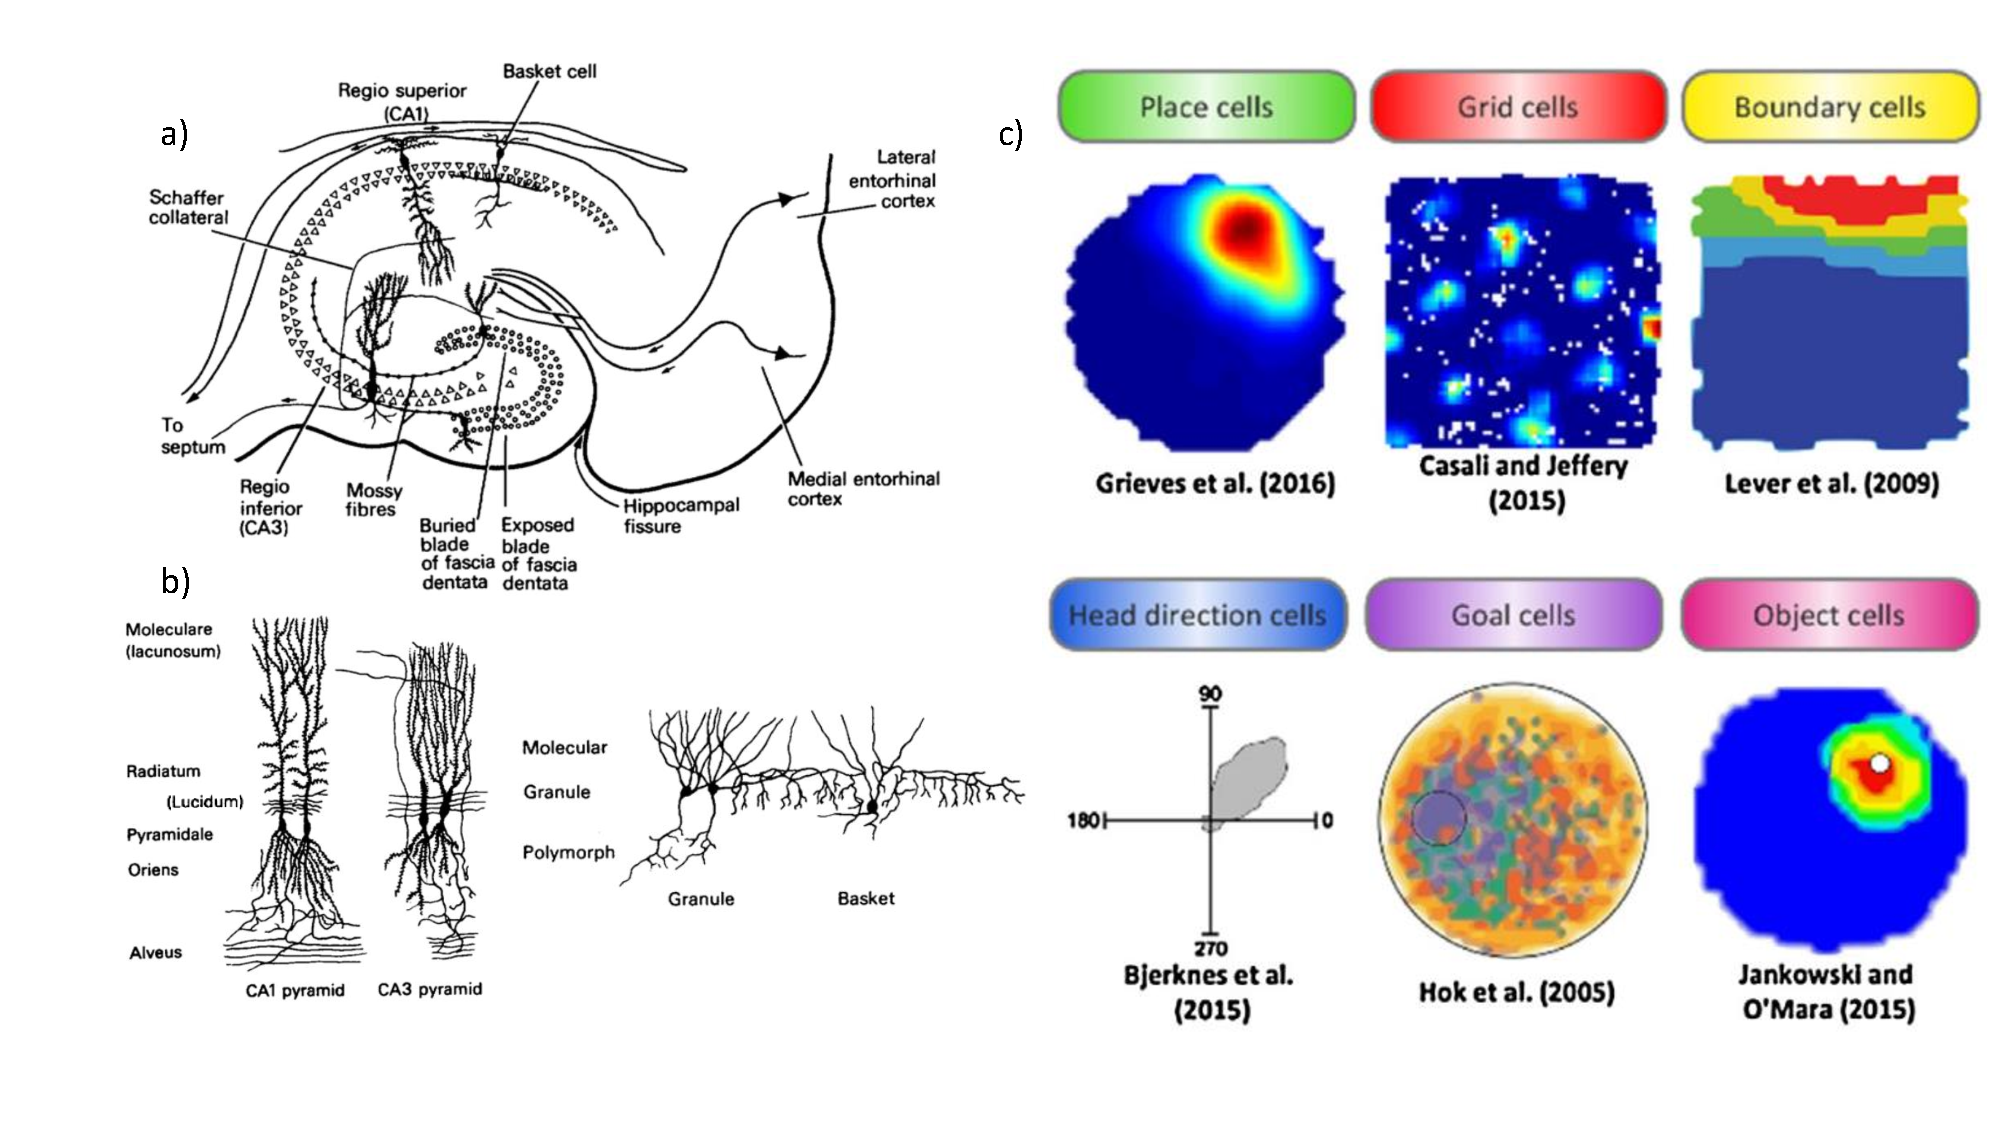
\includegraphics[width=\textwidth]{Figures/Chapter1/intro_fig1.pdf}
    \caption{Hippocampal anatomy and spatial information encoding cells. a) Schematic representation of the mouse hippocampus and the connections between regions, adapted from [REF to okeef book]. b) Examples of CA1 and CA3 pyramidal cells (after Cajal 1911, Fig. 475) and of dentate granule and basket cells of Cajal (after Lorente de No 1934, Fig.10). c) Examples of the different types of spatial information encoding cells that conform the cognitive map, references in place.}
    \label{fig:chap1:spatialnavigation}
\end{figure}

% =========================================================== %
%      Subsection: Spatial information encoding cells         %
% =========================================================== %
\subsection{Spatial information encoding cells}
\label{chap1:sec:1:subsec2:spat_info_cells}
The first type of cells that conform the cognitive map were found by O’Keefe and Dostrovsky in 1971, when electrophisiological recordings in the hippocampus led to the discovery of cells that would fire predominantly in a specific location of a familiar environment.
This cells were called \textit{Place cells}. 
It's impossible to summarize here all what is currently known about place cells, so we will focus only in the main characteristics of this and the rest of the cell types of the cognitive map.

\textbf{Place cells} are mainly found in the hippocampus proper and their firing rate is modulated purely by spatial location, that is, they fire maximally when the animal's head is in a specific region of the environment [Figure \ref{fig:chap1:spatialnavigation}c top-left]. 
This region is called the \textit{place field} of the cell.  
Here we use the term environment in a generic way, but place cells have been mainly studied in constrained laboratory environments.
Interestingly, place cells have different characteristics depending on the nature of the space the animal explores.
Place cells fire at their place field location, regardless of directions of motion or speed when the animal is in a two-dimensional space, like the square/rectangular or circular boxes used in the early O'keefe experiments, but when exposed to a linear track, or one-dimensional environment, place cells would have a preferred direction of firing, and would fire much less or not at all or in a different location when the animal runs in the oposite direction [McNaughton et al., 1983; O’Keefe and Recce, 1993].
Place cells have also been found in three-dimensional environments, having three-dimensional place fields.
The latter type of place cell has been observed in bats flying through a familiar environment [Yartsev and Ulanovsky, 2013], and more recently in rodents exploring three-dimensional environments [Grieves...Jeffery 2020].

The way place cells represent position is not limited to the firing rate of the cells but also to the temporal aspect of their firing. 
Place cell firing is locked to the phase of the sinusoidal local field potential (LFP), called theta rhythm, and hence to the population activity in the hippocampus. 
The theta rhythm works as a sort of clock against which the network can measure time and temporally locate cell spikes allowing place cells to identify locations in an environment with much finer precision than if only rate codes were used.
This is called \textit{Temporal coding} [O’Keefe and Recce (1993), Huxter et al., 2003, György Buzsáki, Andreas Draguhn 2004, Buzsáki 2002].

Nearby place cells do not necessarily have nearby place fields, furthermore, a group of close by place cells would typically have place fields that span the whole space, suggesting that place cells represent a complete and highly redundant representation of the surface [O’Keefe, 1976; Wilson and McNaughton, 1994].
Once formed, these representations are stable across days [Hill, 1978; Muller et al., 1987] or even weeks [Thompson and Best, 1990].
Although, more recently, it has been suggested that not all place fields are stable [Mankin et al., 2015; Ziv et al., 2013]. 

There's a large portion of literature related to what are the necessary inputs to the hippocampus for a place cell to fire. 
This is still an unsolved question, althought there are some clear hints. 
It is clear that visual information is important, as distal cues or landmarks surrounding the environment can influence place field formation [Muller and Kubie, 1987; O’Keefe and Conway, 1978; Yoganarasimha and Knierim, 2005] but it is not necessary. 
Place cells would fire in the same location in the dark in a familiar environment [Save et al., 2000; Zhang et al., 2014; Markus et al., 1994; Quirk et al., 1990], provided that other sensory cues are avialable such as olfaction or tactility. 
All this different modalities are integrated outside of the hippocampus [Jeffery, 2007], which shows that place fields are higher order representations that integrate more primitive spatial constructs such as direction, self motion and boundaries, which again talks about the inputs to the hippocampus. 
If the sensory cues show that the environment has changed or is completly new, a new and unique representation would be formed by the place cells [Anderson and Jeffery, 2003; O’Keefe and Conway, 1978] in a process called remapping [Muller and Kubie, 1987]. 
Importantly, in rats and mice, the animal has to explore the space directly for place cells to form a spatial representation [Rowland et al., 2011], unlike other mammals like primates that can form inferred allocentric representations of remote space if observed [Rolls, 1999; Rolls et al., 1997; Rolls and O’Mara, 1995]. 

So far we've used a rather vague definition of place cell. 
Traditionally, to define a place cell and its place field several criteria related to the firing rate, consistency of firing or reliability were used. 
Here and throughout this work we will define a place cell as a cell in the hippocampus proper that carries \textit{significant amount of information} about the animals position in it's firing activity (see methods). Later on we will define what this means in this context and how we establish significance.  

The second key cell type in the spatial representation are the \textbf{head direction cells} [Figure \ref{fig:chap1:spatialnavigation}c bottom-left].  
Head direction cells are cells in the presubiculum whose firing is modulated, as the name implies, by the facing direction of the head.
They were first found by Rank [Rank 1985, 1984] and described in detailed a few years later [Taube et al., 1990a, 1990b, 1987].
Here \textit{head direction} refers to the orientation of the head in the horizontal plane.
Head direction cells are very similar in their characteristics to place cells: they have a prefer direction of firing that is independent of other behavioural factors; each head direction cell has a different preferred direction; all together, preferred directions are equally distributed in the circle, in the sense that there's no overall preferred direction of the network [Taube et al., 1990b].
Like with place cells, angular orientation of environmental cues are an important modulator of head direction cells activity [Goodridge and Taube, 1995; Taube, 1995a; Taube et al., 1990b; Zugaro et al., 2000Knierim et al., 1995] but are by no means necessary [Mizumori and Williams, 1993; Yoder et al., 2011a,b].
An interesting characteristic of this cells is that the angular relationship between preferred directions of different cells is preserved [Skaggs et al., 1995; Yoganarasimha and Knierim, 2005].
Hence when remapping an environment or if the animal is disoriented and one cell changes its orientation, the rest of the cells change theirs coherently.

With place cells and head direction cells, the cognitive map is able to build positions and to measure angles. 
The next requirement for the map to work is a way of measuring distances, to establish the metric of the map.
In 2005 a cell type that could achieve this task was found in the Moser's lab: the \textbf{grid cells}. 
Grid cells are cells that fire in multiple discrete and regularly spaced locations which form a triangular or, equivalently, an hexagonal lattice [Figure \ref{fig:chap1:spatialnavigation}c top-middle]. 
This cells are found in the medial entorhinal cortex (mEC) and postrhinal cortex [Fyhn et al., 2004; Hafting et al., 2005, Fyhn et al., 2008] and in the pre- and para-subiculum [Boccara et al., 2010]. 

Grid cells have some similar characteristics to place cells or head direction cells.
Their pattern of firing arises in familiar environments and partially relies on distal visual cues; if the environmental cues rotate, grid patterns do so too consistently [Hafting et al., 2005]; and deformation of the environments implies deformation of he patterns [Barry et al., 2007; Stensola et al., 2012].
Like head direction cells, the angles and distances between grid patterns of different grid cells are preserved, and when the environment rotates or moves, the patterns adapt in a coherent fashion, mantaining a stable relationship [Fyhn et al., 2007].
This suggests that grid cells work cooperatively, as an interconected matrix known as attractor network [McNaughton et al., 2006].
Moreover, the spacing between peaks of grid patterns varies as a function of location in the entorhinal cortex. 
The scales of the patterns increase in discrete jumps as one goes from dorsal to ventral in the entorhinal cortex [Vegard Heimly Brun, et al. 2008].
Each animal can have 3 or 4 different scales. 

Finally, we have the \textbf{boundary cells}.
With yet another highly descriptive name, boundary cells, or boundary vector cells, are cells in the subiculum that respond purely to environmental boundaries [Figure \ref{fig:chap1:spatialnavigation}c top-right].
Interestingly, the existence of boundary cells was first hypothesized after the observation that after elongating one side of a rectangular box, place fields would stretch accordingly [O’Keefe and Burgess, 1996].
This led a number of researchers to think that there could exist cells that would fire in relation to environmental boundaries, and that place cells firing could arise as a thresholded sum of a subpopulation of such cells [Barry et al., 2006; Burgess et al., 1997; Hartley et al., 2000]. 
Cells that fit such description, at least partially, were later found in several regions of the brain, like the subiculum [Barry et al., 2006], presubiculum and parasubiculum [Boccara et al., 2010], mEC [Bjerknes et al., 2014; Savelli et al., 2008; Solstad et al., 2008] and recently in the anterior claustrum [Jankowski and O’Mara, 2015] and rostral thalamus [Jankowski et al., 2015].

More formally we could define boundary vector cells as cells that fire when the animal encounters an environmental boundary in it's preferred direction.
And it's firing is driven by the memory of the boundary's position related to the animal, based not only on perceptual cues, but also on self motion information [Lever et al., 2009; Raudies et al., 2012; Raudies and Hasselmo, 2012]. 
This definition requires that we clarify two things: first, what is a boundary? A boundary can be walls, low ridges or vertical drops and the colour, texture or odour of these does not seem to influence the cell’s firing [Lever et al., 2009].
Second, what does it mean to \textit{encounter} a boundary? Cells would fire at a specific distance from the boundaries, and this distance is different for cells in different brain regions [Bjerknes et al., 2014; Solstad et al., 2008, Jankowski and O’Mara, 2015, Lever et al., 2009].

Place cells, head direction cells, grid cells and boundary vector cells lie at the core of the cognitive map and represent the most relevant and more studied type of cells in the context of spatial navigation. 
However the further the cognitive map and the greater hippocampal formation is studied, the more \textit{types} of cells are found. 
Cells with more abstract or complex firing patterns, cells that respond to clear real-world correlates, but also cells that respond to more abstract or conjunctive correlates. 
We will not describe them here, but in this list we should mention \textbf{object cells}, \textbf{goal cells}, \textbf{boundary-off cells}, \textbf{perimeter cells} and \textbf{band cells}, among others. 

It's interesting to think how each of this cell types can arise, due to which inputs, and in which combinations.
In other words, what is the relation between the firing patterns of all these cell types?
Mathematically is easy to show that place cells can be formed by summing two grids of different spacing, or equivalently by summing two border cells, or that grid cells can be built by combining band cells.
The function and structure of each of this firing patterns is not yet understood.
It is however almost difficult to believe that the brain builds such an explicit and interpretable map, using specialized cells in trackable combinations.
This is of course, just the tip of the iceberg and the more the extended hippocampal formation is studied, the more cell types and complicated firing patterns appear. 

However, as intense and productive all the before-mentioned (and much more that has not been mentioned here) research has been in the last decades, we can't help but to notice that it concerns only a subgroup of the full brain network: the neurons.
But neurons represent approximately half of the cells in the brain, depending on the species can be more or less, the rest are \textbf{Glial cells}.
Although glial cells don't have electrical activity like neurons have, they express rich calcium dynamics and interact with cells in active ways. 
In this work we will approach the question of if and what role play glial cells in spatial navigation in the mouse brain. 

But first we will briefly describe the types of Glia cells that can be found in the brain, focusing specially on \textbf{Astrocytes}, the main actor of this work,  their characteristics and the recent literature regarding its calcium signaling and its role in modulating neuronal activity. 

% =========================================================== %
%                      Section: Glia                          %
% =========================================================== %
\section{Glia}
\label{chap1:sec2:glia}
Glial cells have been first observed as early as the mid $19^{th}$ century by Virchow [Virchow, 1856], and better described and brought to wider attention by Santiago Ramón y Cajal and Pío del Río Hortega a few decades later thanks to the development of chloride-sublimate technique, a staining technique that targets specifically astrocytes.
At the time, glial cells were thought to play a strictly structural role in the brain.
If anything else, the terminology used to describe them would be sufficient to understand the hypothesized role: described as \textit{Zwishchenmass}, german for \textit{inbetween mass}, \textit{Nervenkitt}, or \textit{nerve glue} in english, and finally the current terminology \textit{Glial cell} comes from the Greek word \textit{gl\'ia} meaning \textit{glue}.
It wasn't until the second half of the $20^{th}$ century when electrophysiological characterization and physiological studies of glial cells permitted the understanding of the wide range of vital functions that glial cells have in the functioning of the central nervous system [Morrison and de Vellis, 1981, Bowman and Kimelberg, 1984; Kettenmann, Backus and Schachner, 1984, Cornell-Bell et al., 1990a, Araque et al., 1998; Bezzi et al., 1998]. 
Phylogenic studies show that all organisms with a central nervous system have glial cells, and, interestingly, the ratio of astrocytes-to-neurons is different depending on the animal species and on the brain region, with intriguing correlates with brain complexity and neuronal density [Herculano-Houzel, 2011, Herculano-Houzel, 2014].   
Throughout evolution, glial cells have diverge into specialized subgroups with different characteristics and function. 
The total glial population can be divided into four major groups: \textbf{microglia}, \textbf{astrocytes}, \textbf{oligodendrocytes} and their progenitors \textbf{NG2-glia}. 

Unlike the rest of the glial cells, \textbf{Microglia} originate from yolk-sac progenitors that only populate the brain during development [reviewed in Kim and de Vellis, 2005; Kettenmann et al., 2011].
They represent the main immuno-competent and phagocytic cells of the central nervous system [Filiano AJ, Gadani SP, Kipnis J August 2015], and cover the major part of adult brain in individual non-overlapping domains.
Microglia sense the environment through the movement of their filopodia, which rapidly reacts to abnormalities or damage [Nimmerjahn et al., 2005; Cronk and Kipnis, 2013].
Besides the inmuno-role, microglia has recently been hypothesized to have an active role in the healthy brain. 
Opinions on this matter are, however, controversial. 
While some studies show that microglia could be involved in motor-dependent synapse formation [Parkhurst et al. (2013)] and in features as high order as learning or social behavior [Torres et al., 2016, Kierdorf and Prinz, J Clin Invest. 2017], others have shown that ablation of microglia barely produce any alterations or pathologies in healthy adult mice [Elmore et al., 2014, 2015; Bruttger et al., 2015].
This discrepancies might be due to the major methodological differences in each study [Sarah Jäkel,and Leda Dimou 2017].

\textbf{Oligodendrocytes} are a type of large macroglia cells first observed by Pío del Río Hortega in the first half of the $20^{th}$ century.  
Their function is somewhat more clear: they insulate axons with self-produced myelin to allow a fast saltatory conduction and give trophic support to axons [reviewed in Nave, 2010].
However oligodendrocytes have been found in sparsely myelinated brain regions, this presumably non-myelinating oligodendrocytes might have other functions that have been so far overlooked.

More interesting are the more recently discovered oligodendrocytes precursors, the \textbf{NG2-glia} cells [ffrench-Constant and Raff, 1986].
Their first more evident function is that of forming and maintaining a homeostatic network, preserving the cell numbers stable by generating mature myelinating oligodendrocytes throughout lifetime [Dimou et al., 2008; Rivers et al., 2008; Psachoulia et al., 2009; Simon et al., 2011, Hughes et al., 2013] under physiological conditions.
What's really interesting about the NG2-glia cells is their ability to form functional synapses with neurons.
A fenomena first observed in the hippocampus [Bergles et al., 2000] but later described in other brain regions [Karadottir et al., 2005; reviewed in Sun and Dietrich, 2013].
Such synapses are uniderectional in the sense that can only receive neuronal sygnals but can't generate action potentials on their own and further propagate them [De Biase et al., 2010].

The last large group of glia cells in the brain are the \textbf{Astrocytes}.
Astrocytes and the effect of alterations on their calcium activity represent the main focus of this thesis. 
For this reason we will spend the next few sections on describing their function, anatomy and their known relation with neuronal activity. 

% =========================================================== %
%                    Subsection: Astrocytes                   %
% =========================================================== %
\subsection{Astrocytes}
\label{chap1:sec:2:subsec1:astrocytes}
Astrocytes are the most abundant type of glial cell and represent up to $40\%$ of all the cells in the mammalian brain [Herculano-Houzel, 2014].
Despite being one of the first glial cells to be discovered around 150 years ago, their description and the understanding of their role in the brain function is far from complete.
As with everything in biology (is getting annoying really), astrocytes do not represent single homogeneous cell type and can be subdivided into several types depending on their morphology, molecular profile or function. 

From the morphological point of view astrocytes can be roughly divided into two types: \textbf{fibrous} and \textbf{protoplasmic}.
The first one is a star-shaped cell with regular contours present mainly in the white matter of the brain and spinal cord and in the optic nerve and the retina fiber layer.
Fibrous astrocytes are characterized by their elongated morphology, with long processes running parallel to the axon bundles that make contact with myelinated axons and with oligodendrocytes.
They have fewer processes compared to protoplasmic astrocytes.
Their processes spatially overlap in their domains and extend to perivascular, subpial and axonal endfeet [Lundgaard et al., 2014].

Protoplasmic astrocytes on the other hand have a “bushy” and irregular morphology, with a small round somata of $\sim 10 \mu m$ in diameter.
Present $5-10 \sim 50 \mu m$ primary processes, that further branch into thousands of branchlets and leaflets that form dense arborisations that connect with synapses [Bushong et al., 2002], and large endfeet that in turn connect with the vasculature [Nagelhus and Ottersen, 2013; Verkhratsky, Nedergaard and Hertz, 2015].
Unlike fibrous astrocytes, protoplasmic astrocytes populate mainly the gray matter in the brain and have domains with well defined borders that do not overlap between each other [Bushong et al., 2002].
Even when the the area of influence of an astrocyte is limited to local domains and do not mix with other astrocytes, it is highly connected and has a strong influence in neuronal activity.  
A single astrocyte arborisation can cover 20,000 to 80,000 $\mu m^3$, contacting 300 to 600 dendrites and potentially 100,000 individual synapses [Bushong et al., 2002, Halassa et al., 2007].
This dense connectivity allows astrocytes to control several processes like ion homeostasis or neurontransmitter recycling.
Interestingly, astrocytic domain boundaries have been proposed to be determined by, or at least closely relate to, neuronal functional units [Perea, Sur and Araque, 2014].
In this sense astrocytes could play the role of controlling and modulating \textit{functional islands} formed by the synapses confined within the area of influence of a single astrocyte [Halassa et al., 2007].
Further supports this hypothesis the fact that branching and connectivity of astrocyte, even from the same type, strongly depends on brain region.  
When comparing striatal and hippocampal astroglial populations it was noted that, despite having the same somatic volume, equivalent number of primary branches, and the same total cell volumes, hippocampal astrocyte territories are more constrained and display a tighter physical interaction with excitatory synapses [Chai et al., 2017] compare to striatal ones.

If astrocytes are so closely related to neuronal function and, as said before, have big and dense areas of influence, what are astrocytes functions in the brain? 
This question represents still a very active area of research. Here we will enumerate some of the known functions that astrocytes fulfill but will later describe in more detail the role of astrocytes in modulating neuronal activity. 

Astrocytes are involved in the \textbf{control of cerebral blood flow} through \textbf{gliovascular coupling}.
Matching the blood flow to the neuronal metabolic needs is crucial for healthy brain functioning, this is achieved by astrocytes in a two-fold manner. 
First by regulating dilation of blood vessels: it has been proved that synaptic activity mediates cytoplasmic calcium increases in astrocytes, that in turn promote dilation of neighbouring arterioles [Zonta et al., 2003, Attwell et al., 2010].
At the same time, astrocytes regulate vasoconstriction through the release of 20-hydroxyeicosatetraenoic acid (20-HETE) [Zonta et al., 2003, Metea and Newman, 2006].
Interestingly, astrocytes seem to \textit{decide} weather to drive dilation or constriction based on local oxygen levels and metabolic states [Macvicar and Newman, 2015]. 

Given the enormous energy consumption in the brain, the regulation of oxygen and glucose availability must be tightly controlled.
This is, of course, in part regulated by blood flow. However, while oxygen freely diffuses in the brain, glucose and other metabolites need specialised transporters to travel through cell membranes.
The need for energy depends on neuronal activity, that can go from completely silent to high firing rate in miliseconds, which in turn can demand up to 30-fold increase in metabolic consumption [Attwell and Laughlin, 2001]. 
It has been demonstrated that astrocytes, who are in contact both with blood vessels and synapses, strongly and tightly control active \textbf{metabolic support} to neurons. 
This can be achieved through a variety of processes that are still an intense area of study. 
Glucose is preferentially taken by astrocytes rather than neurons [Pellerin et al., 2007], that enters glycolysis and produces lactate.
Lactate is then delivered to neurons via the astrocyte-neuron lactate shuttle (ANLS) [Pellerin and Magistretti, 1994)]. 
Meaning that astrocytes are not only involved in the metabolic support of neurons through blood flow regulation but also through direct delivery of energy substrates. 

Astrocytes, together with microglia, have a key role in the \textbf{immune response} of the brain, both in physiological and pathological conditions.
Upon brain injury or disease, astrocytes become reactive, drastically changing gene expression and entering full metal fight mode [Zamanian et al., 2012].
This changes induce morphological and functional alterations that lead astrocytes to enter one of two distinct reactivity profiles, depending on the nature of the insult. 
Inflammatory insult leads astrocytes to enter what has been called \textit{A1}, a reactivity profile implied in synapse pruning suggesting a detrimental role.
On the other hand, ischemic injury leads to activation of reactivity profile \textit{A2} responsible for growth and survival of neurons and synapses, indicating a protective role. 
Such contrasting mechanisms coexisting in the same cell type proves once more, the complexity, diversity and specificity of astrocytic function. 
Moreover, in physiological conditions, astrocytes continue to play a role in immune protection of the brain by maintaining the blood-brain barrier (BBB). 
Interestingly, astrocytes have been shown to be involved in BBB formation during development [Hayashi et al., 1997]. 

Besides the aforementioned functions, astrocytes play key roles in Ion [Sibille, Pannasch and Rouach, 2014, Nwaobi et al., 2016], water [Nielsen et al., 1997, Risher, Andrew and Kirov, 2009] and neurotransmitter [Danbolt, 2001, Herman and Jahr, 2007] homeostasis. 
Astrocytes can rapidly change their volume and intercellular communicative capacity, which allows them to redistribute water across astrocytic networks.  
Can redistribute $K^+$ ions through $K^+$ spatial buffering, and are the only cells in the central nervouse system that can synthesize glutamate and GABA from glucose. 
Astrocytes are an incredible versatile and complex cell that account for an incommensurate amount of functions and roles in the brain, however the aspect of astrocytes that concerns this work relates to the signaling in astrocytes and its relation with neuronal activity. 
We will discuss this aspects next. 
% =========================================================== %
%        Subsection: Calcium signaling in astrocytes          %
% =========================================================== %
\subsection{Calcium signaling in astrocytes}
\label{chap1:sec:2:subsec1:astro_calcium_signals}
As inexpert scientists, we PhD students have a bias view of the way research works towards positive discoveries and confirmed hypothesis. 
Simply because our biggest source of information are publications, and the chances of getting a story published that states "\textit{we formulated \textbf{this} hypothesis, and found it to be wrong}" are very low, there's a lack of charm in failure that prevents unsuccessful hypothesis to be known. 
Which is regrettable, because proven wrong hypothesis are at least as informative as positive results.
With brilliant examples like the Michelson-Morley experiment in 1887, where the two physicist trying to prove the existence of the aether, the medium in which light was thought to propagate, proved instead that it didn't exist.  
And in the way invented the interferometer. 
Invention that was later crucial for the development of the special theory of relativity and, more recently, for the detection of gravitational waves.
We can go even further and say that logic allow us \textit{only} to falsify theories, but, on the other hand, to prove a theory \textit{correct} is impossible. 
We can get encouraging results, experiments that help us gain confidence in our working hypothesis, but not really prove it.
On the other hand, one counterexample is all that is needed to prove it wrong.
As Einstein eloquently put it: \textit{The scientific theorist is not to be envied. For Nature, or more precisely experiment, is an inexorable and not very friendly judge of his work. It never says "Yes" to a theory. In the most favorable cases it says "Maybe," and in the great majority of cases simply "No." If an experiment agrees with a theory it means for the latter "Maybe," and if it does not agree it means "No." Probably every theory will someday experience its "No"—most theories, soon after conception.} [Albert Einstein: the human side: New glimpses from his archives. Dukas and Hoffman 1922]
Perhaps a way to compensate for this bias is to get rid of the miss-conception that falsifying an hypothesis represent failure but instead call it for what it is, a scientific discovery.  

In a way, a fruitful, but less interesting substitute of self-falsified hypothesis are the stories of scientist trying to prove \textit{other} peoples theories wrong, because controversy, unlike failure, sells journals.
One of the highly interesting and still active controversies in neuroscience is the question whether calcium concentration elevations in astrocytes regulates neuronal and vascular function.
This has led in the last few decades to a series of works by different groups that appeared to be contradictory, and different research lines have been seemingly proving each other wrong to give rise to a better and more profound understanding of the subject.  
We will not refer here the complete story that has been brilliantly summarized by Bazargani and Attwell [Bazargani and Attwell 2016], but will refer only some characteristics of calcium signaling in astrocytes that are relevant for the understanding of this work.

It's important to note first, that astrocytes, unlike neurons, are non-excitable cells.
For this reason, $Ca^{2+}$ fluctuations have been considered as the main intracellular readout of detection of environmental changes.
That includes astrocyte-neuron communication. 
An extensive amount of work in the last few decades has been dedicated to understand the origin of $Ca^{2+}$ transients, if this fluctuations are somehow relevant for neuronal regulation, and if so, how.
To the date most of this questions remain unanswered, although currently there seems to be a common consensus in the field that (spoiler alert) they are at least involved in several regulation pathways, and respond, in physiological conditions to behavioral and sensory correlates. 

Should caught our attention the fact that baseline levels of $Ca^{2+}$ in astrocytes are higher than that of neurons, and that this concentration vary inside each cell, being higher in processes compared to the soma [Zheng et al., 2015].
Which already suggest two observations: first, the relevance of $Ca^{2+}$ in astrocytic signaling, and second, the within-cell complexity of it. 
In astrocytes, $Ca^{2+}$ fluctuations can have different sources, the first of which is intrinsic. 
In fact, it was shown that $65\%$ of astrocytes in hippocampal slices exhibit asynchronous and localised $Ca^{2+}$ transients, even in the absence of neuronal activity [Nett et al., 2002].
The role and relevance of these untriggered events has yet to be defined. 
Specially because it's unclear if this spontaneous events do happen in physiological conditions and if so, in which fashion. 

More interesting are \textbf{$Ca^{2+}$ changes induced by neuronal activity}.
Glutamate has been shown to evoke calcium concentration rise in astrocytes in several contexts, in culture [Cornell-Bell et al., 1990], in brain slices [J.W. Dani et al., 1992], in whole retina [Newman and Zahs 1997] and \textit{in vivo} [Wang et al. 2006].
This calcium transients can propagate along astrocyte processes and even between glial cells [ornell-Bell et al., 1990, J.W. Dani et al., 1992, Hirase, H. et al., 2004, Nimmerjahn, A. et al., 2004].
This observations further support the possibility that glial Ca2+ waves might constitute an extra-neuronal signaling system in the CNS, and, importantly, that it can be driven by neuronal activity. 
However, to begin to understand the neuron-astrocytic $Ca^{2+}$ activity relation one must realize that, just like neurons, astrocytes have to be thought as the sum of many different subcellular compartments and that calcium transients occurring in the soma are very different and can have different sources as the the ones in fine astrocytic processes near synapses.
$Ca^{2+}$ events in processes can occur independently of larger ones in the soma, which suggest that regulation of synapses or blood vessels can happen locally. 
This events can, however, propagate to neighbouring intracellular areas [Di Castro et al., 2011] or even synchronise with neighbouring cells [Takata et al., 2013].
Importantly, it has been shown that such events correlate with the strength of neuronal activity [Panatier et al., 2011].

Process and soma $Ca^{2+}$ events also differ in their temporal profile.
While is true that somatic calcium transients are several order of magnitude longer than neuronal action potentials, which has been an historical argument against the hypothesis that astrocyte could be involved in real-time information processing in the brain, smaller events occur in processes even in the subsecond scale [Winship, Plaa and Murphy, 2007; Lind et al., 2013, 2018].
This partially solves the temporal argument, but in a more fundamental aspect, it's by no means clear if information processing in neuronal network relies in temporal or rate coding or a combination of both.
Rate coding responses could be an alternative way in which long lasting astrocytic $Ca^{2+}$ signals could be involved in a relevant temporal scale in neuronal activity and information processing [Semyanov, 2019].
On a further bigger scale, $Ca^{2+}$ events can propagate as waves through networks of several tens and even hundreds of astrocytes.
Behavior that  has been observed in cultures [Cornell-Bell et al., 1990b], as well as \textit{in vivo} in the frontal and parietal cortices upon sensory stimulation []Ding et al., 2013] and in the cerebellum during locomotion [Nimmerjahn, Mukamel and Schnitzer, 2009].
Giving rise to the possibility of astrocytes modulating neuronal activity at a network scale. 

As stated before, many of such calcium transients have been shown to depend, or have its origin in neuronal activity dependent processes. 
In hippocampal dentate gyrus astrocytes action potential–driven synaptic transmitter release triggers large and long lasting ($\sim3 s$), spatially broad ($\sim12 \mu m$) events, while spontaneous synaptic transmitter release produces brief ($\sim 0.7 s$), spatially localized ($\sim 4 \mu m$) transients [Di Castro, M.A. 2011].
It has been suggested that release of $Ca^{2+}$ from internal stores could be the main source of $Ca^{2+}$ somatic transients, while in the astrocyte processes transmembrane entry of $Ca^{2+}$, presumably through endogenously active channels such as TRPA1 [Shigetomi, 2012] or receptor-gated $Ca^{2+}$-permeable ion channels, generates 30–40\% of $Ca^{2+}$ concentration elevations. 
In this way while $Ca^{2+}$ rises in astrocyte somata may be too slow [Schummers, et al. 2008, Schulz, K. et al, 2012] to generate rapid blood flow increases, $Ca^{2+}$ transients in the processes that are faster than in the soma [Tang, W. et al. 2015] occur before or with a similar time course to the increase of blood flow [Lind, B.L. 2013, Otsu, Y. et al, 2015].

We will not dig into the specific mechanisms through which neuronal activity could induce such calcium transients (related to the activation of mGluR receptors by glutamate release) or the controversies involved. 
But will instead mention some of the observations that evidence astroctytic calcium transients physiological relevance. 
It has been observed that whisker stimulation increases $Ca^{2+}$ concentration in astrocytic cytoplasm in the barrel cortex [Wang et al., 2006], in a frequency dependent manner [Perea and Araque, 2005; Sherwood et al., 2017]. Other behavioural variables like locomotion or arousal state have been observed to evoke $Ca^{2+}$ elevation over broad spatial areas, mediated by noradrenaline signals in the frontal and parietal cortex [Ding et al., 2013, Paukert, et al., 2014].
Suggesting an astrocytic involvement in the control and modulation of sensory input and behavior. 
% =========================================================== %
%   Subsection: Astrocityc modulation of neuronal activity    %
% =========================================================== %
\subsection{Astrocityc modulation of neuronal activity}
\label{chap1:sec:2:subsec2:astro_neuromodulation}
The complexity both in source and dynamical properties of calcium oscillations in astrocytes makes it rather complicated but at the same time extremely interesting to study.
We've seen that astrocyte calcium changes are related to neuronal activity, to neurotransmitter release and to sensory input and behavioral state.
That they can occur in fast transients in the processes or in longer, stronger events in the soma. 
That can propagate within the cell, across neighbouring cells and through extended networks.
This covers one way of information flow in the \textit{extended brain network} (that is considering neurons and glial cells). 
But what is the role (or roles), if any, of each of this astrocytic calcium dynamics in the processing of information by neuronal networks?
In other words, how does astrocytic activity modulate neuronal functioning?
We are interested in the answers to this questions that are related to the brain information processing and its meaning for behavioural outputs, and therefore to the astrocytic-induced changes in neuronal properties. 

Given that astrocytes extend processes that are ideally positioned for dynamic exchange with the synapses, the first observations are related to how astrocytes influences synapses. 
This happens in three aspects: by regulating \textbf{presynaptic release probability}, \textbf{postsynaptic receptor activation} and \textbf{synaptic plasticity}.
Importantly, release of gliotransmitters, which is one of the key ways in which astrocytes comunicate with neurons, is widely accepted to follow cytoplasmic $Ca^{2+}$ rise in astrocytes, making $Ca^{2+}$ transients highly relevant for the comunication between neurons and astrocytes and its experimental testing.
However, we have to keep in mind that gliotransmitters can have different effects depending on the target, the neuronal activity regime, the brain region, and the developmental state to be able to properly interpret the extended network activity. 

At the \textbf{presynaptic level}, it has been observed that in the dentate gyrus, astroglial glutamate release activates presynaptic NMDA receptors, potentiating excitatory transmission [Jourdain et al., 2007].
Similarly, in the hippocampus proper glutamate potentiate transmitter release, although in this case by activating presynaptic mGluRs but without the intervention of NMDA receptos [Perea and Araque, 2007; Navarrete and Araque, 2010].
Astrocyte release of glutamate has been observed to mediate not only excitation but also inhibition at the presynaptic level during sustained neuronal activity.
This is achieved in two ways, first by binding presynaptic kainate receptors that strengthen inhibitory synaptic transmission [Kang et al., 1998; Liu et al., 2004], and second, $Ca^{2+}$ uncaging-mediated glutamate release from astrocytes produce binding of presynaptic mGluRs in neurons that in turn decrease evoked postsynaptic currents in the hippocampus [Araque et al., 1998].
It has been recently shown that single astrocyte may release different gliotransmitters [Covelo and Araque, 2018], which can induce more complex modulation of synapses: high frequency stimulation of the CA3-CA1 projection in the hippocampus produced finely tuned release of both glutamate and adenosine from astrocytes, modulating synapses in a biphasic way.
Initial glutamate release induced potentiation followed by purinergic-mediated depression of neurotransmitter release, which represents an elegant example of the subtle and complex modulation effects of neuronal comunication by astrocytes. 

At the \textbf{postsynaptic level} it has been observed that disrupting gliotransmission in a dnSNARE mouse model produced a hypofunction of postsynaptic NMDA receptors, which has effects at the network level affecting cortical slow oscilations (see bellow) [Fellin et al., 2009].
Similarly NMDA receptors binding have been shown to be modulated by astroglial D-serine release, which in turn modulates glutamatergic synaptic transmission [Panatier et al., 2006, Henneberger et al., 2010].

Astrocyte gliotransmission has been observed to have effects in \textbf{synaptic plasticity} and memory.
Clamping $Ca^{2+}$ in individual CA1 astrocytes blocks LTP inductions at nearby excitatory synapses by decreasing the occupancy of the NMDAR co-agonist sites [Henneberger et al., 2010].
Exogenous D-serine or glycine application reverse this effect.
Note that this $Ca^{2+}$-dependent release of D-serine from an astrocyte control of NMDAR-dependent plasticity can potentially affect many thousands of excitatory synapses but only those that are nearby, implying a local regulation of neuronal activity. 
This further advocates for the functional spatially localized aspect of astrocytic domains.   
Conversely, astrocytes can also modulate synaptic depression. 
$Ca^{2+}$ clamping in rat barrel cortex astrocytes during development showed impaired t-LTD [Min and Nevian, 2012].
Moreover, simultaneously stimulating an astrocyte with depolarising pulses and afferent fibres resulted in LTD.
This result suggests that astrocyte signalling is sufficient to induce plasticity at the level of neuronal synapses. 
Finally, astrocytes have been shown to be involved in the synaptic depression of untetanised synapses paralleling LTP in the hippocampus [Pascual et al., 2005; Serrano et al., 2006; Andersson, Blomstrand and Hanse, 2007; Chen et al., 2013]

There are several mechanisms through which astrocytes modulate \textbf{neuronal excitability}, that is, neuronal electrical dynamics during action potential firing. 
Action potentials or spikes in neurons depend on the fine and complex relation between ionic concentrations withing neurons and in the extracellular space, which is in turn regualted by the activity of voltage-gated ion channels.
One of the most consolidated functions of astrocytes is the maintenance of ionic homeostasis and more specifically the buffering of extracellular potassium [Kofuji and Newman, 2004, 2010; Kimelberg and Nedergaard, 2010; Hertz and Chen, 2016].
The rapid intake of $K^+$ by astrocytes prevents neuronal hyperexcitability [Bellot-Saez et al., 2017]. 
Although the specific intracellular mechanisms are not clear, there has been strong evidence towards the idea that astrocytes, through the secretation of purines set neuronal firing thresholds, both in pyramidal cells and interneurons [Kawamura, Ruskin and Masino, 2010, Kawamura et al., 2004, Tan et al., 2017].

We mentioned how astrocytes modulate each side of the synapse and synaptic plasticity and later how they influence neuronal excitability. 
Continuing with the growing scale progression, astrocytes play key roles in the \textbf{synchronization of neurons} and at the \textbf{network level}.
As we stated at the beginning of this section, the mechanisms through which astrocytes influence neuronal activity depend on cell type, brain region and developmental state of the animal.
In the absense of neuronal activity hippocampal CA1 neurons present inward currents with slow kinetics found to be mediated by glutamate released from astrocytes, simillar to those observed under stimulation of Schaffer collaterals [Fellin et al., 2004].
This response occurs synchronously in multiple CA1 neurons, evidencing the functional role of astrocytes in the synchronization of neurons.
More recently, it has been observed that cellular coordination might not involve inter-astroglial Ca2+ spread, suggesting other mechanisms of astroglial networks cell coordination [Chever et al., 2016]. 
However, neuronal network oscilations or brain waves are not restricted to the hyppocampus, instead they are present in almost every brain region, during sleep, sensory perception, can have functions that vary from memory consolidation to temporal coding (as mentioned before) and lie in a wide variety of frequency and power bands.   
The mechanisms by which network oscillations are formed and modulated are still a matter of intense study.
Interestingly, it has been recently proposed that astrocytes might play a role in the regulation of neuronal membrane potential oscillations at a wide range of frequencies [Bellot-Saez et al., 2018].
Indeed blockade of $K^+$ uptake or astrocytic connectivity, enhance network excitability and form high power network oscillations.
This could be due to changes in the oscillatory behaviour of individual neurons, which is a well known effect in the system dynamics field.
More precisely it has been shown that, as we mentioned before, impairing gliotransmission altered slow wave dynamics in the cortex by reducing neuronal depolarization periods duration, and prolonging hyperpolarization [Fellin et al., 2009].
Moreover, slow oscillations involves oscilation in neuronal membrane potential as well as astrocytic calcium dynamics, with the latter preceding neuronal changes.  
And alterations in astrocytic calcium dynamics inhibits slow wave activity, showing the fine causal interplay between both types of cells during brain oscillations [Szabó et al., 2017].
Finally, astrocytic signaling has been observed to be involved not only in gamma oscillations but also in their cognitive correlates [Lee et al., 2014], being this an example of how astrocytes acitivity is crucial for proper performance in tasks as high order as novel objet recognition.

We couln't and wouln't try to make a full description of the vast plethora of mechanisms by which neurons and astrocytes interact, or the function of each of this interactions, many of which are a matter of active debate to date. 
Heterogeneity in experimental procedures might account for some of the discrepancies in the literature.
But we hope we've built so far the case that astrocytes, and in particular astrocytic $Ca^{2+}$ dynamics, is involved and regulates the way the brain process information.
It does so at the level of the synapses, in single cells, and at the network scale.
That this interactions go both ways, with astrocytes modulating neuronal dynamics but also neuronal activity interfering in astrocytic profiles.
That the complexity and richness of this modulation extends not only to the spatial domain but also at the temporal scale, with small fast and local interactions as well as large waves of activity spanning whole brain regions.
And more important, that when studying the way the brain solves a task, considering only neuronal networks might not be enough, and a shift in the paradigm towards the study of an extended neuronal-glial networks might be needed. 

% =========================================================== %
%        Subsection: Astrocytes accumulate evidence           %
% =========================================================== %
\subsection{Astrocytes accumulate evidence}
\label{chap1:sec:2:subsec4:astro_evidence}
So far we've discuss how astrocytes are involved in the way in which neurons process information, focusing mainly in the mechanisms by which such interactions might take place.
However, to further develop the idea of the brain acting as an extended network of both neurons and glial cells during the processing of information, we are inclined to ask the complementary question whether astrocytes or astrocytic networks process information themselves, and if so, how. 

The pursuit of the answer to this question has produced very recent findings that bring some light to the matter, as well as pose more questions. 
Misha Ahrens group studied the interplay off astrocytic and neuronal networks during swimming adaptation strategies and information integration in larval zebra fish [Yu Mu, et al., 2019]. 
In this task animals were exposed to a virtual reality environment where visual feedback was eventually decoupled from motor actions so that the swim behaviour would fail to trigger the expected visual flow. 
The animals, after becoming aware of the futility of their efforts would became passive and stop motion, to then try again a few seconds later. 
When animals switched from the active to the passive behavioral state, whole-brain average neuronal activity decreased while glial activity increased. 
In this case, activity refers to $Ca^{2+}$ transients that started seconds before and peak after passivity onset. 

The availability of chemical, optical and genetic tools allows interventional approaches that can test this hypothesis from a causal point of view. 
Reduction of astrocytic $Ca^{2+}$ activity by two-photon laser ablation of glial cells or blocking the inositol 1,4,5-trisphosphate receptor to reduce Ca2+ release from intracellular stores, led to a reduction in  futility-induced passivity. 
Using a chemogenetic approach to increase intracellular $Ca^{2+}$ in glia on the other hand led to an increase in the time spent in passive state. 
This effect was temporally tuned as shown by optogenetic activation (either using CoChR or Opto-a1-AR). 
Which suggests that astrocytic $Ca^{2+}$ are necessary and sufficient for the expression of this behavior. 

Interestingly, the way astrocytes exert this effect on behavior is achieved through a finely tuned interplay between neuronal and astrocytic networks. 
More precisely during futility-induced passivity, signals from noradrenergic (NE) neurons together with local circuit activity triggered glia responses as proved by optogenetically activating NE neurons. 
Showing that astrocytes integrate both behavioral information as well as NE signals.
Astroyctes, in turn, activated GABAergic neurons that would most likely supress swimming. 

The question that interests us the most is what is the \textit{information} processing that is done in each step of this complex behavior by each element of the network? 
Through a series of complex but very elegant probabilistic experiments, the group demonstrated that NE neurons signals encode sensory-motor mismatch signal.
Signals that are transmitted to astrocytes that in turn \textit{accumulate evidence} that actions are futile and control, through GABAercig neurons, swimming behavior. 

This example beautifully puts together several of the functions and characteristics of astrocytes discussed previously in a orchestrated mechanisms with a behavioural output with high level of complexity. 
It shows in a physiological and behavioural relevant way, how astrocytes are involved in network state changes, how they integrate neuronal activity, modulate downstream circuits, influence behavior and importantly, process information in complex and functional ways.  
It evidences how to uncover the underlying functional role of astrocytes it is sometimes necessary to see the big picture and perform experiments and tasks closer to ethological behaviours.  

Only days ago, another elegant example of how astroyctes are involved in complex behavior modulation has been published [Seungwoo Kang, 2020]. 
The group showed that in mice, astrocytes from the dorsomedial striatum differentially regulate medium spiny neurons activity facilitating shifts from habitual to goal-directed reward-seeking behavior.
And they do so by tuning excitatory and indirect inhibitory postsynaptic currents in neurons, process regulated by adenosine metabolism, receptor signaling, and transport. 
This examples manifest, however, the complexities of the experimental procedures needed for proper understanding of network functioning during complex behaviors \textit{in vivo}.
% ================================================================ %
% Section: Astrocytes encode spatial information in Ca2+ activity  %
% ================================================================ %
\section{Astrocytes encode spatial information in $Ca^{2+}$ activity}
\label{chap1:sec3:astro_spat_info}
Finally we'll summarize recent unpublished work from our lab, that settled the basis for the work in this thesis.
As we've seen, astroyctes are involved in the processing of information in the brain, both by encoding specific aspects of behavioural variables and the relation with the environment and by interacting with neuronal networks. 
Astrocytes and their interactions with neurons have been extensively studied in the hippocampus [Perea and Araque, 2007, Pascual et al., 2005; Serrano et al., 2006; Andersson, Blomstrand and Hanse, 2007; Chen et al., 2013, Covelo and Araque, 2018], however as discussed in the first part of this introduction, one of the most interesting and thoroghly studied functions of hippocampal networks is the encoding of spatial information and the building of a cognitive map for spatial navigation.
The question whether hippocampal astroctyes intervene, alter or modulate spatial information encoding in neurons or, more fundamentally, if navigational information is encoded exclusively in neuronal cells or it involves the extended brain network comprising glial cells as well as neurons had not been elucidated to date. 
Our lab has tackled this question by specifically asking how astrocytic calcium signaling relates to spatial navigation, with the working hypothesis that astrocytes encode navigational information in their intracellular calcium dynamics. 

There are, however, a few remarks that are needed to understand the following results and the research exposed in this thesis.
So far we have been talking about \textit{information}, \textit{information flow} or \textit{encoding of information} in a rather loose way, without defining what we really mean. 
However, throughout this work, \textbf{information} will have a very well defined and concrete meaning, and that is the one established by \textbf{information theory}.
We'll explain these concepts in the next few paragraphs.

Information theory was first developed by C. E. Shannon and beautifully exposed in his landmark paper \textit{A Mathematical Theory of Communication} [Shannon 1948].
In it, Shannon develops a mathematical formalism of communications, considering the coding an decoding problem of information in noisy channels.
This theory has extended to many fields with several practical and theoretical applications, notably modern computation, quantum mechanics, quantum computation and neuroscience.
There are several ways of approaching the notion of information as in Shannons theory, we will expose a modified version of the one exposed in his paper.
We'll take his approach first because it relates information to probability distributions in an intuitive way which is what we need, second because of its comprehensibility and third because, in a slightly more abstract sense, the brain can be thought as a noisy communication network, with neurons being both transmitters and receivers.
However, it's useful to keep in mind what's the objective, what is it that we are trying to use information theory for. 
The question we'll try to answer is: if we look at neuronal activity, how much information do we gain from a certain behavioral variable (for example the position of the animal)? 

Lets try to formalize the problem: neurons can be in several states, depending on how we describe them. 
We can think of a neuron as a variable with two states, either firing or not, or with a continuum of states, like all the possible values of its membrane potential or of the calcium concentration inside the cell.
Lets consider then in a general way that each state of the neuron has a certain probability, namely state $x$ has probability $p_x$ of occurring.
When we observe a neuron we gain information about its state, the neuron was either firing or not. 
However before measuring it we can ask the question of \textbf{how uncertain are we about the state of the neuron if we know the set of probabilities $\{p(x)\}$}.
This is equivalent to asking the question of \textit{how much} information we gain when we learn the state of the neuron. 
In this example we are using the state of a neuron, but the approach is general to any probability distribution.
To answer a 'how much' question (either uncertainty we have or information we gain) we need a quantitative measure, lets call this measure $H$.
There are three rather reasonable properties that we'd like to ask of $H$:
\begin{itemize}
    \item \textbf{$H$ should be a function only of the probabilities}, it doesn't matter if it's neuron 1, 2 or Z, if it's a principal neurons or an interneuron (or an astrocyte) as long as the probabilities of its states are the same, therefore we can write $H(p_x)$.
    And \textbf{$H$ should be continuous in $p_x$}.
    \item If all the events are equally possible, that is $p_i=\frac{1}{n}$ with $n$ the amount of states, then \textbf{$H$ should be a monotonic increasing function of $n$}.
    Intuitively, if there are more possible states, and all the states are equally possible, there is more uncertainty.
    \item The information gained when two independent events occur with individual probabilities $p$ and $q$ is the sum of the information gained from each event alone.
\end{itemize}
It can be proved that the only $H$ that satisfies all three properties is of the form: 
\begin{equation}
    H=-K \sum_{x=1}^n p_x\ log (p_x)
\end{equation}
with $K$ a positive constant that amounts only to the choice of units of measure.
This expression might ring a bell for those who have studied statistical mechanics, $H$ is nothing but the \textbf{entropy}. 
We select the logarithm to be in base $2$ (all logarithms in this thesis will be in base $2$ unless otherwise specified), which is achieve by appropriately selecting the constant $K$, and define the entropy of the probability distribution $p_1,p_2,...,p_n$ of an n state variable as:
\begin{equation}
    H=- \sum_{x=1}^n p_x\ log_2 (p_x)
\end{equation}
This definition is intuitive but is not the whole story. Probably the best reason to define entropy in this way is because it can be used to \textit{quantify the resources needed to store information}. 
It can be proved that Shannon's entropy represents the minimal physical resources required to store the information being produced by a source, in such a way that at a later time the information can be reconstructed.
This result is known as the \textit{Shannon’s noiseless coding theorem}.

It might be useful to build a toy example to illustrate some of the properties of $H$. Lets consider an overly simplified neuron with two possible states, it can be either firing or not. It fires with probability $p$ and is silent with probability $q=1-p$, then its entropy is given by
\begin{equation}
    H=-(p\ log (p) + (1-p)\ log (1-p))
\end{equation}
We can see the values of $H$ as function of $p$ in the figure \ref{fig:chap1:info_theory_concepts}a.
If the neuron would always be silent and never fire, we'd have no uncertainty of its state and we would gain no information by measuring its state.
In this example that is represented by $p=0$ and therefore $H=0$.
If, on the other hand, the neuron would fire randomly half of the time, we would have absolute uncertainty about its state before measuring and therefore we'll gain the maximum amount of information after measurement.
That is, its probability of firing would be $p=0.5$ and the entropy would be $H=1$.
Meaning that knowing the state of the neuron gives us $1$ bit of information.
In general we have that $H=0$ if and only if all $p_i=0$ except one that is $1$, and the uniform distribution is the probability distribution with maximum entropy and the entropy is the logarithm of the number of states.
That is $H=log(n)$ and is maximum if and only if $p_i=\frac{1}{n} \; \forall \ i$.

Now, before we tackle the question that brought us to this point to begin with, we have to define other important quantities from the theory.
Let's say we have another variable with its own states and probability distribution ${p(y)}$, that can represent another neuron, or set of neurons, or a behavioral variable like the position of the animal. 
We define the \textbf{joint entropy} of variables $X$ and $Y$ as
\begin{equation}
    H(X,Y)\equiv-\sum_{x,y}p(x,y)\ log(p(x,y)) 
\end{equation}
The joint entropy measures our total uncertainty about the pair $(X,Y)$.
Now, suppose we learn the value of $Y$, meaning that we gained $H(Y)$ bits of information about the pair $(X,Y)$.
How much uncertainty remains about the pair $(X,Y)$? 
Or in other words, how uncertain are we about $X$, given that we know the value of $Y$?
This quantity is called the \textit{entropy of $X$ conditional on knowing $Y$} and is defined as
\begin{equation}
\label{eqn:condentropy}
    H(X\ |\ Y) \equiv H(X,Y)-H(Y)
\end{equation}
Now we have everything we need to define the quantity that would answer our initial question that was: if we look at neuronal activity, how much information do we gain from a certain behavioral variable (for example the position of the animal)? 
We can reformulate this question into an analogous form and ask, how much information is shared between neuronal activity and the behavioral variable?
In a general way, lets consider two variables $X$ and $Y$, suppose we add the information content of $X$, $H(X)$ to the one of $Y$, $H(Y)$.
If there's information shared in the two variables, then we will be counting it twice, and information that is not common will be counted only once. 
So if we subtract then the total amount of information of the pair, which is nothing but the joint entropy $H(X,Y)$ what will remain is the common or the \underline{\textbf{mutual information}} of $X$ and $Y$:
\begin{equation}
\label{eqn:mutualinfo1}
    I(X:Y)\equiv H(X)+H(Y)-H(X,Y)
\end{equation}
In the last paragraph we have been using \textit{information} and entropy as interchangeable concepts.
That is because, as we said at the beginning of this section, entropy quantifies the amount of uncertainty about a variable before knowing its state or equivalently, how much \textit{information} we gain when we measure its state.
However, we could arrive to the expression for mutual information in a slightly different but equivalent way that might be more reassuring about the use of the term \textit{information}.
Recall that \textit{conditional entropy} $H(X\ |\ Y)$ represents the uncertainty that remains in $X$ given that we learned the value of $Y$.
Thus, the complement of the uncertainty that remains is the \textit{information we gained} about $X$ by knowing $Y$. Formally, we can define \textit{mutual information} then as 
\begin{equation}
\label{eqn:mutualinfo2}
    I(X:Y)\equiv H(X) - H(X\ |\ Y)
\end{equation}
The equivalency of this two expressions \ref{eqn:mutualinfo1} and \ref{eqn:mutualinfo2}
is trivially shown simply by replacing \ref{eqn:condentropy} in \ref{eqn:mutualinfo1}.
The various definitions and relationships between entropies might be difficult to picture or remember. 
A useful way of visualizing them is using the 'entropy Venn diagram' shown in figure \ref{fig:chap1:info_theory_concepts}, which is not completely reliable as a guide of the properties of entropy but can provide a comprehensible mnemonic. 

Information theory has been widely used and studied in neuroscience.
With works as early as Richmond and Optican in the 1990 [Richmond and Optican, 1990] on the primate visual cortex or Skaggs formula for spiking activity in 1993 [Skaggs et al., 1990].
There are several reasons for the success and usefulness of information theory approaches for studying the brain.
First, information theory is model independent, in the sense that we are not required to explicitly specify what is our model of the interaction between the variables of our system.
This does not mean that information theory is \textit{assumptions} free, in general there are several assumptions we have to do about the data, for example it is required to assume the data to be stationary, i.e. if a neuron is encoding information about a behavioral variable at the beginning of the experiment, it will do so at the end.     
Second, because of its probabilistic nature, information theory is applicable regardless of the data type, meaning that we can use it if one of the variables is represented by a binary signal like the case of spikes in a neuron, or if its the continuous variable of speed of an animal in $cm/s$.
Third, information theory can uncover non-linear relations between variables.
And finally, all the quantities presented so far are easily scalable to many variables, therefore applicable to many neurons or a neuron and several behavioral variables, etc.

As with anything in life, it does come with its perks and considerations and has to be used with care and a proper understanding of the tools.
This is particularly true when dealing with real data, because, although very solid and versatile in its formalism, information theory requires the knowledge of the underlying probability distributions of the variables, which is never really known. 
Probably the stronger assumption that we do then to use information theory for real data is that we can get an empirical approximation of the underlying probability distribution, and that it is a good approximation. 
The bias implied by using empirical probability distributions has been extensively studied and several alternatives for correcting such bias have been proposed [Panzeri et al., 2007, Panzeri and Treves 1995].

Information theory approaches have been traditionally used for studying spiking trains, and therefore electrophysiological data [Skaggs 1993].
However as we said before, this approach can be used regardless of the nature of the data types, more recently it has been used for analyzing information content and correlations in calcium activity as recorded by 2-photon imaging [Shuman et al., 2020, Stefanini et al., 2020, Rubin et al., 2015, Sheintuch et al., 2017].

\begin{figure}
    \centering
    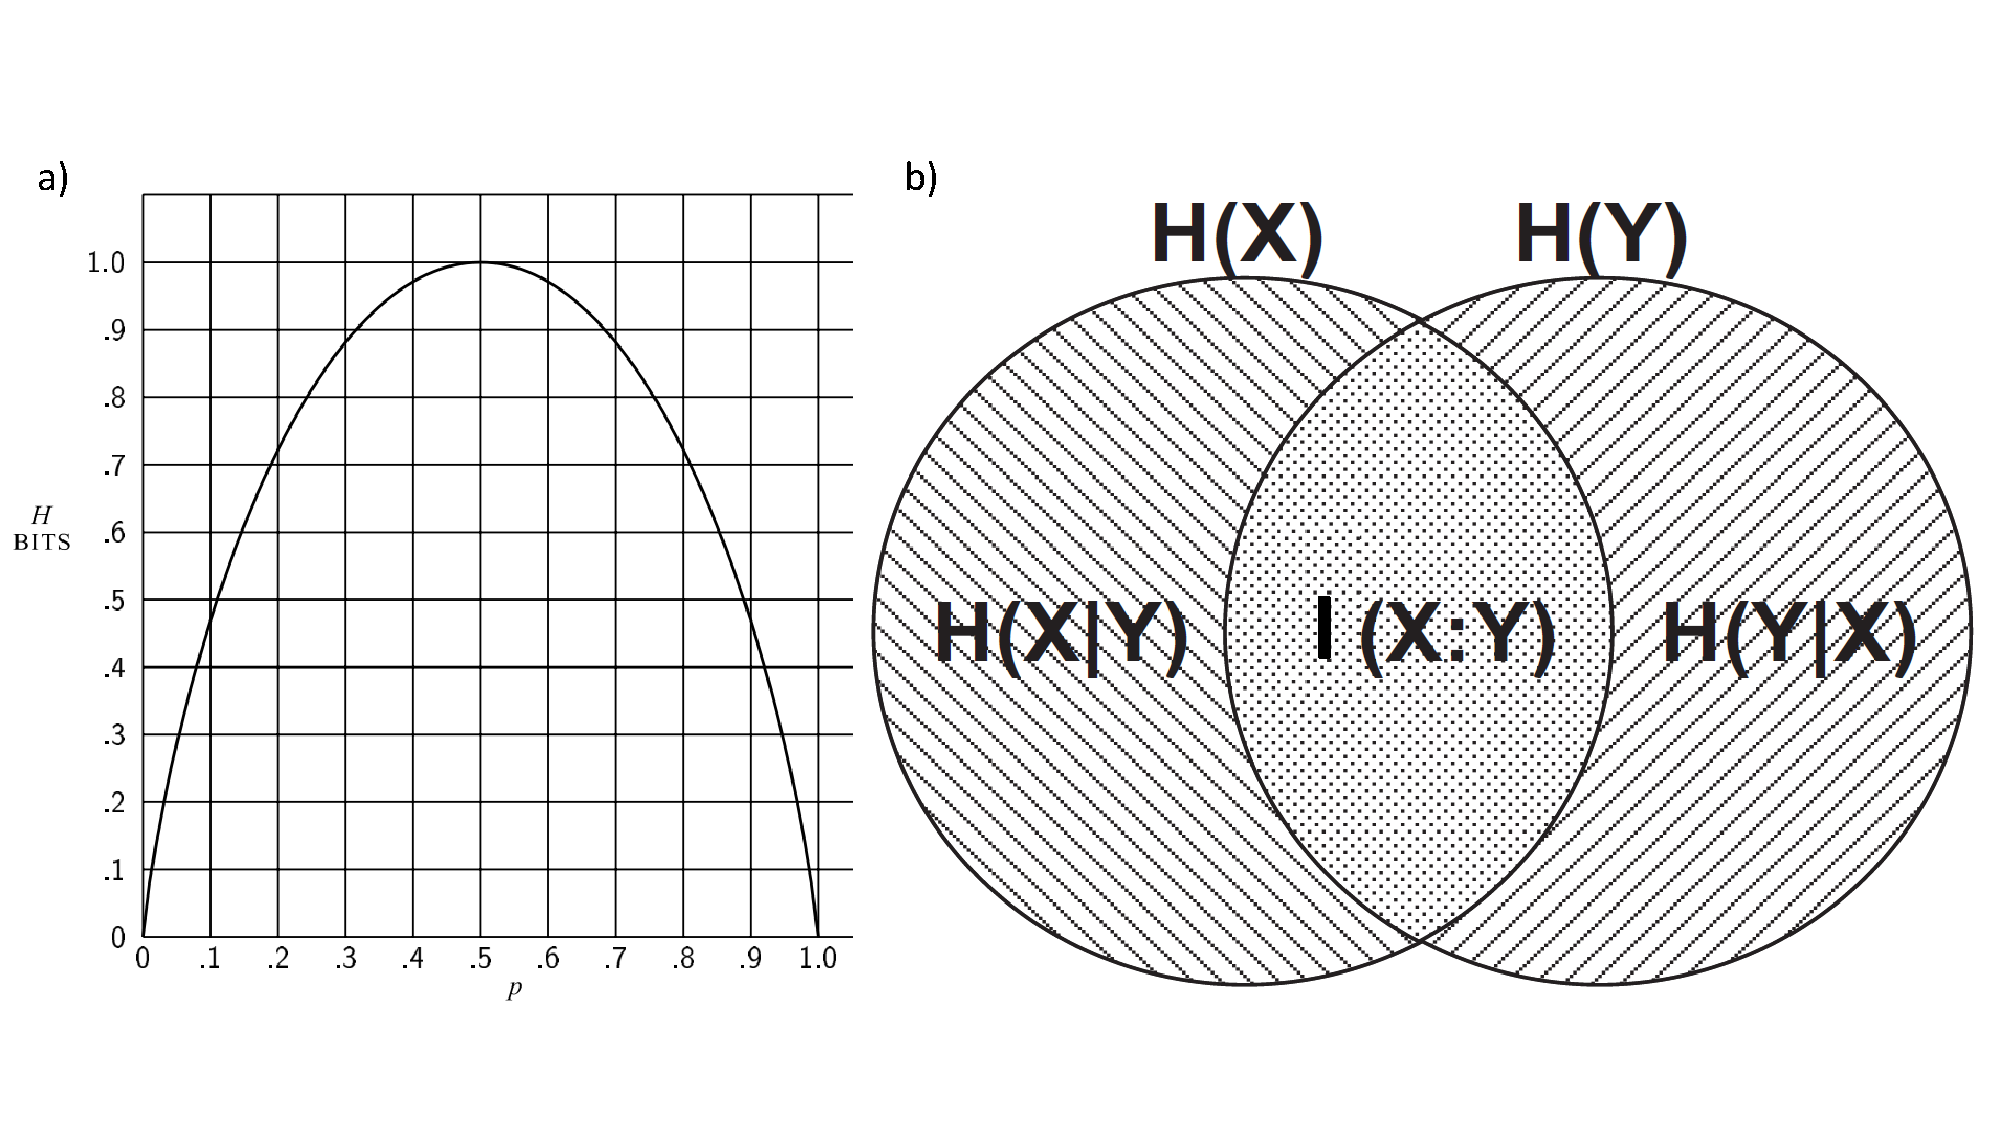
\includegraphics[width=\textwidth]{Figures/Chapter1/intro_fig_info.pdf}
    \caption{Concepts of entropy and information theory. a) Entropy of a binary variable as a function of the probability $p$, adapted from Shannon 1948 b) Schematic entropy and information Venn diagram, adpated from Nielsen and Chuang book, 2010.}
    \label{fig:chap1:info_theory_concepts}
\end{figure}
% =========================================================== %
%        Subsection: Astrocytes and information               %
% =========================================================== %
\subsection{Astrocytes and information}
\label{chap1:sec:3:subsec1:astro_info}
In the context of information theory, the first question was whether astrocytes encode information about the position of the animal.
To answer this question, mice where trained to run head-fixed in a virtual reality corridor [Figure \ref{fig:chap1:sebapaper}a] [Gauthier and Tank 2018].
Using astrocyte-specific expression of the genetically encoded calcium indicator GCaMP6f [Chen; Khakh] together with two-photon functional imaging to capture subcellular calcium dynamics of hippocampal CA1 astrocytes, it was found that that a fraction of astrocytic regions of interest (ROIs) carried significant information about the spatial position of the animal in the virtual track [Figure \ref{fig:chap1:sebapaper}b,c].
In this context \textit{significant amount of information} is related to how the mutual information value compares to surrogate distributions of MI values build by temporally shuffling the data (see methods for details). 
Broadly speaking, this astrocytes show calcium activity that could be interpreted as the glial analogous to the spiking activity of place cells, thus, it is adequate to define the spatial response field of the informative astrocytes and study their characteristics.
It was shown that the distribution of field positions covered the entire length of the virtual corridor [Figure \ref{fig:chap1:sebapaper}d left], suggesting a full map of the environment, done by astrocytes, parallel (or complementary) to that of the neuronal network.
Similar to neurons, when exposed to a bidirectional environment, astrocytic ROIs showed significant direction selective spatial modulation in their response field.

Following the discussion from previous sections, it is interesting to see if this coding is intrinsic to astrocytic processes, somas or both. 
It was found that both cell bodies and processes encoded spatial information and that a larger fraction of somas than processes were modulated by the spatial position of the animal [Figure \ref{fig:chap1:sebapaper}d right].
Unlike neurons, the preferred position of astrocytes was not entirely random.
This was observed first because correlation between the calcium activity of pairs of informative ROIs decreased as a function of the pair distance [Figure \ref{fig:chap1:sebapaper}e top].
And second, because the difference between the field position of the two informative ROIs in a given pair increased as a function of the pair distance within $0-40 \mu m$ and reached a constant value, indicating that informative calcium signals were coordinated across cells [Figure \ref{fig:chap1:sebapaper}e middle].
Similarly, when looking at the single cell level, the difference between the field position of an informative process and the corresponding somas increased as a function of the process distance from soma [Figure \ref{fig:chap1:sebapaper}e bottom], demonstrating that spatial information is differentially encoded in topological distinct locations of the same astrocyte. 
\begin{figure}[t]
    \centering
    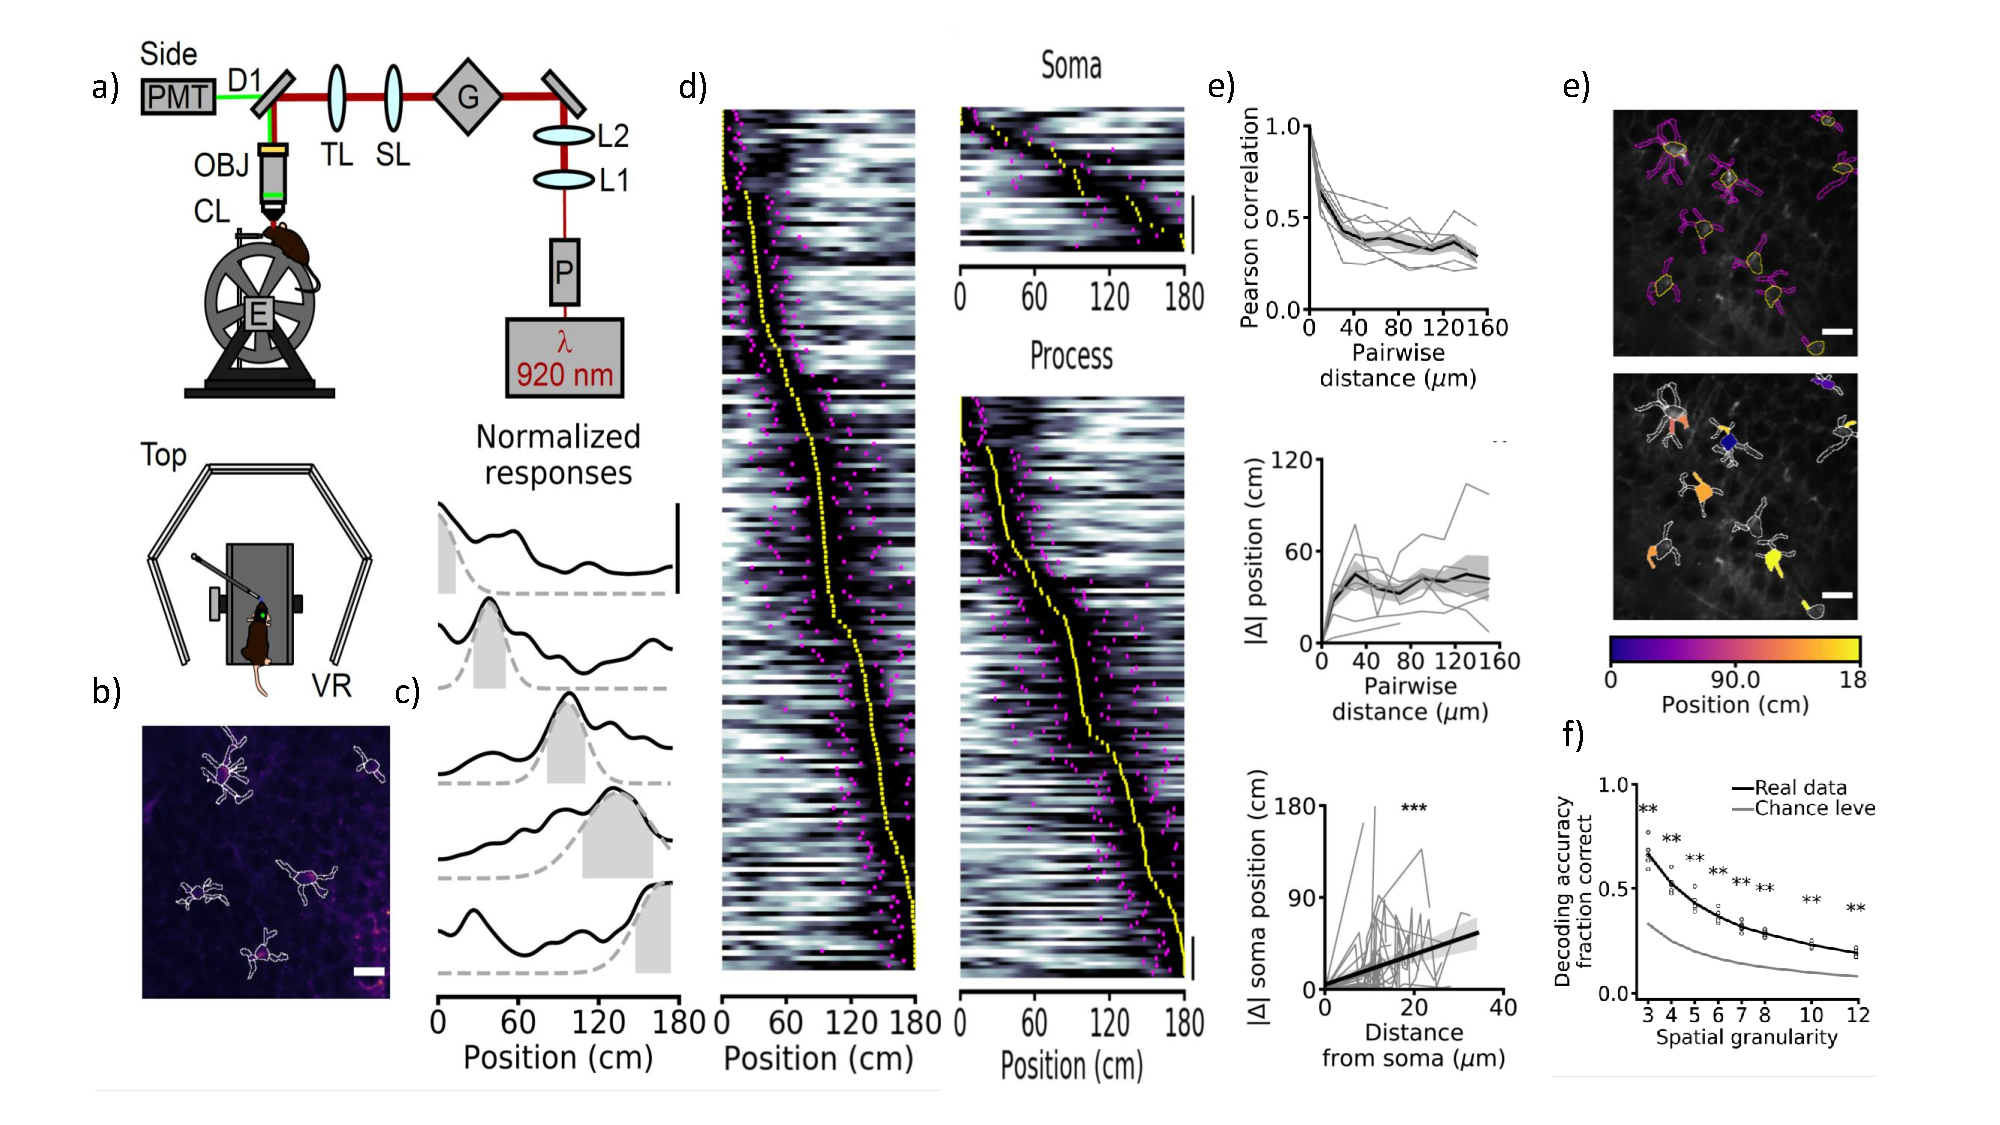
\includegraphics[width=\textwidth]{Figures/Chapter1/intro_fig_seba.pdf}
    \caption{Calcium dynamics in astrocytes networks in the hyppocampus encode spatial information. a) Schematics of the experimental setup, b) example of the 2-photon calcium imaging, c) example traces and modeled place fields, d) normalized astrocytic calcium responses as a function of position for astrocytic ROIs that contain significant amount of spatial information, left all ROIs, top-right somas, bottom right processes. e) Pairwise Pearson’s correlation (top) and difference between response field position (middle) for pairs of astrocytic ROIs across the whole FOV as a function of ROIs pairwise distance. Difference in response field position of a process with respect to the field position of the corresponding soma as a function of the process distance from cell soma (bottom). f) Decoding accuracy as a function of decoding granularity on real (black line) and shuffled (grey line) data.}
    \label{fig:chap1:sebapaper}
\end{figure}
% =========================================================== %
%             Subsection: Decoding of position                %
% =========================================================== %
\subsection{Decoding of position}
\label{chap1:sec:3:subsec2:position_decoding}
We've seen that astrocytes encode spatial information in the hyppocampus, and that a complete map (at least in a uni-dimensional virtual track) could be extracted from the network. Meaning that the place fields of all astrocytes observed span the whole space.
However, is there sufficient information about space in the astrocytic network to infer the animals position? 
To answer this question a support vector machine (SVM) was trained to solve the classification problem of decoding mouse's position using single-trial astrocytic calcium signals according to a set of discrete locations. 
The decoder accuracy, that represents how many times the decoder correctly classify the position of the mouse, was significantly above chance level, regardless of the granularity used in the space domain [Figure \ref{fig:chap1:sebapaper}f]. 
This is important because it means that a downstream neuron (or network) would be able to decode animals position by integrating astrocytic calcium transients information, suggesting the behavioral relevance of it. 

% =========================================================== %
%                    Subsection: Page Margin                  %
% =========================================================== %
% \subsection{Page Margin}
% \label{chap1:sec:2:subsec1:page_margin}
% The format of page size and margin is defined in ``main.tex'' file \textbf{Line 63-71}. The page margin of the current version template is \uline{Left: 35mm, Right: 36mm (a4paper).} Users can change the page margin by adjusting the corresponding settings. There is no stipulation for the top and bottom margins, but the booklet recommend that both of them should be 25mm, which is adopted in this template. 


% =========================================================== %
%          Subsection: Font, Alignment, Line Spacing          %
% =========================================================== %
% \subsection{Font, Alignment, Line Spacing}
% Ordinarily, there is no restrict stipulation for the font family, font size, alignment, and line spacing. All of these are a matter of personal preference. This template uses \textit{10pt} font size, \textit{Fully Justified} alignment style and \textit{One and A Half} line spacing. Users can adjust the settings in \textbf{Line 19-33} of the ``main.tex'' file to change the typeset.


% =========================================================== %
%                      Subsection: Contents                   %
% =========================================================== %
% \subsection{Contents}
% The contents of this template can be subdivided into three parts --- the front matter, the text and the back matter, which strictly follows the stipulations of the official booklet (Page 17). \tabref{chap1:longtable:checking_list} indicates the what contents are required in the submitted thesis and what contents are optional. The column ``Required'' denotes that 
% \begin{center}
% \begin{longtable}{|l|c|c|}
% \caption{Checking list indicating the contents should be included in the thesis.}\label{chap1:longtable:checking_list}\\
% \hline
% \textbf{The Front Matter} & Required     &  Include $\checkmark$ \\ \hline \hline
% Abstract                  & Yes          & $\checkmark$         \\
% Title Page                & Yes          & $\checkmark$         \\
% Frontispiece              &              &                      \\
% Dedication                &              & $\checkmark$         \\
% Epigraph                  &              &                      \\
% Declarations              & Yes          & $\checkmark$         \\
% Acknowledgements          &              & $\checkmark$         \\
% Table of Contents         & Yes          & $\checkmark$         \\
% List of Illustrations     &              &                      \\
% List of Figures           &              & $\checkmark$         \\
% List of Tables            &              & $\checkmark$         \\
% List of Algorithm         &              & $\checkmark$         \\
% List of Abbreviations     &              & $\checkmark$         \\
% List of Symbols           &              & $\checkmark$         \\
% Others                    &              &                      \\ \hline \hline
% \textbf{The Text}         & Yes          & $\checkmark$         \\ \hline \hline
% \textbf{The Reference or Back Matter} &    ---    &   ---       \\ \hline \hline
% Glossary                  &              &                      \\
% Appendices                &              &                      \\
% Notes                     &              &                      \\
% Bibliography or Reference List & Yes          &  $\checkmark$   \\
% Index                     &              &                      \\
% \hline
% \end{longtable}
% \end{center}
% This template support most of the contents listed in the figure, including the ``Abstract'', ``Title Page'', ``Declarations'', ``Acknowledgements'', ``List of Publications'', ``Contents'', ``List of Figures'', ``List of Tables'', ``List of Algorithms'', ``List of Abbreviations'', ``List of Symbols'', ``Main Text'', ``Appendices'', and ``Bibliography''. Each part is defined in an independent tex file and the ``main.tex'' file combines all the different parts to form the entire thesis. Therefore, users can easily make the changes by adjusting the corresponding document files.

% In addition to the stipulations of the booklet, this template also provides a beautiful \textbf{cover page}, which is the first two pages of this project. \uline{The cover page is \textbf{not required} by the Graduate School and you'd better remove the cover page when bounding your thesis for submission.}








